\documentclass[12pt]{article}
\usepackage[margin=1.2in]{geometry}
\usepackage{amsmath}
\usepackage{ctex}
\usepackage{siunitx}
\usepackage{graphicx}
\usepackage{subcaption}
\usepackage{gensymb} 
\usepackage{xcolor}
\usepackage{soul} 
\usepackage{tcolorbox} 
\usepackage{float} 
\usepackage{circledsteps}
\newtcolorbox[auto counter, number within=section]{highlightedsection}[2][]{colframe=cyan!80!black, colback=cyan!30, coltitle=black, sharp corners, fonttitle=\bfseries, title=#2,#1}

\title{实验五\,\,IP调用+蓝牙透传实验报告}
\author{姓名：怀迪\,\, 学号：PB23061112 \\ }
\date{}
 
\begin{document}
\maketitle

% 使用 tcolorbox 使标题带有荧光笔效果
\begin{highlightedsection}{}
    一、实验内容简述
\end{highlightedsection}
本次实验分成两部分，一个是调用IP核实现，调用一个Altera的宏功能模块ROM，
并在ROM中存放正弦波一个完整周期的数据。再编写顶层实体，将ROM模块
当作元件调用，实现一个正弦波产生器。最终的结果采用 Quartus中自带的嵌
入式逻辑分析仪 SignalTap$\prod$来观察；

另一部分是使用蓝牙透传模块，实现串口通信功能，进行从机和主机的数据传输和接收。


\begin{highlightedsection}{}
    二、设计分析
\end{highlightedsection}
\section*{实验题目分析}
\subsection*{1.IP调用实验}
本实验需要自己编写的代码不多，我们仅需要在顶层模块中将存储器
 mystorage 作为元件进行调用即可。

并且在顶层模块中添加一个always语句设计一个计数器，计数值作为存储器
mystorage 的地址，以便mystorage存储器中存储的正弦波数据依次输出。
\subsection*{2.蓝牙透传实验}
本实验主要目的是让我们体验蓝牙透传模块的使用方法，并实现串口通信功能。

我们只需要跟着实验文档的步骤进行连接和配置即可实现两个PC端之间的通信。

\begin{highlightedsection}{}
    三、VHDL源代码
\end{highlightedsection}
\subsubsection*{3.1 IP调用实验}
\begin{figure}[ht]
    \centering
    % 第一张图，宽度 0.45 页宽
    
\includegraphics[width=0.96\textwidth]{代码1.png}
\end{figure}



\begin{highlightedsection}{}
    四、仿真结果记录
\end{highlightedsection}
\section*{1.IP调用实验（蓝牙透传实验无需仿真）}
\begin{figure}[H]  % H 表示固定图片位置
    \centering
    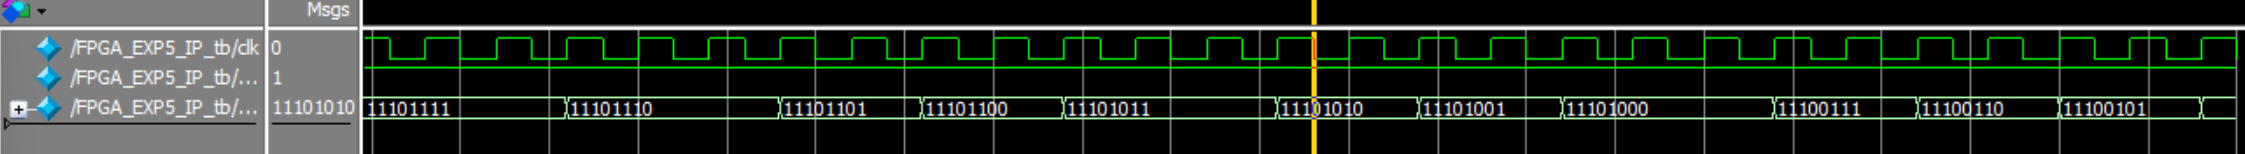
\includegraphics[width=\textwidth]{仿真2.png}  % 图片的最大宽度为文本宽度
\end{figure}
上图为部分仿真波形图，可以看到仿真结果与预期一致，ROM模块
mystorage 中存储的正弦波数据能够正确输出。


\begin{highlightedsection}{}
    五、FPGA验证结果记录
\end{highlightedsection}
\section*{1.IP调用实验}
本实验需要自己编写的代码不多，我们仅需要在顶层模块中将存储器
 mystorage 作为元件进行调用即可。

实验输出结果如下图所示，可以看到输出的波形为一个完整的正弦波周期。
\begin{figure}[H]  % H 表示固定图片位置
    \centering
    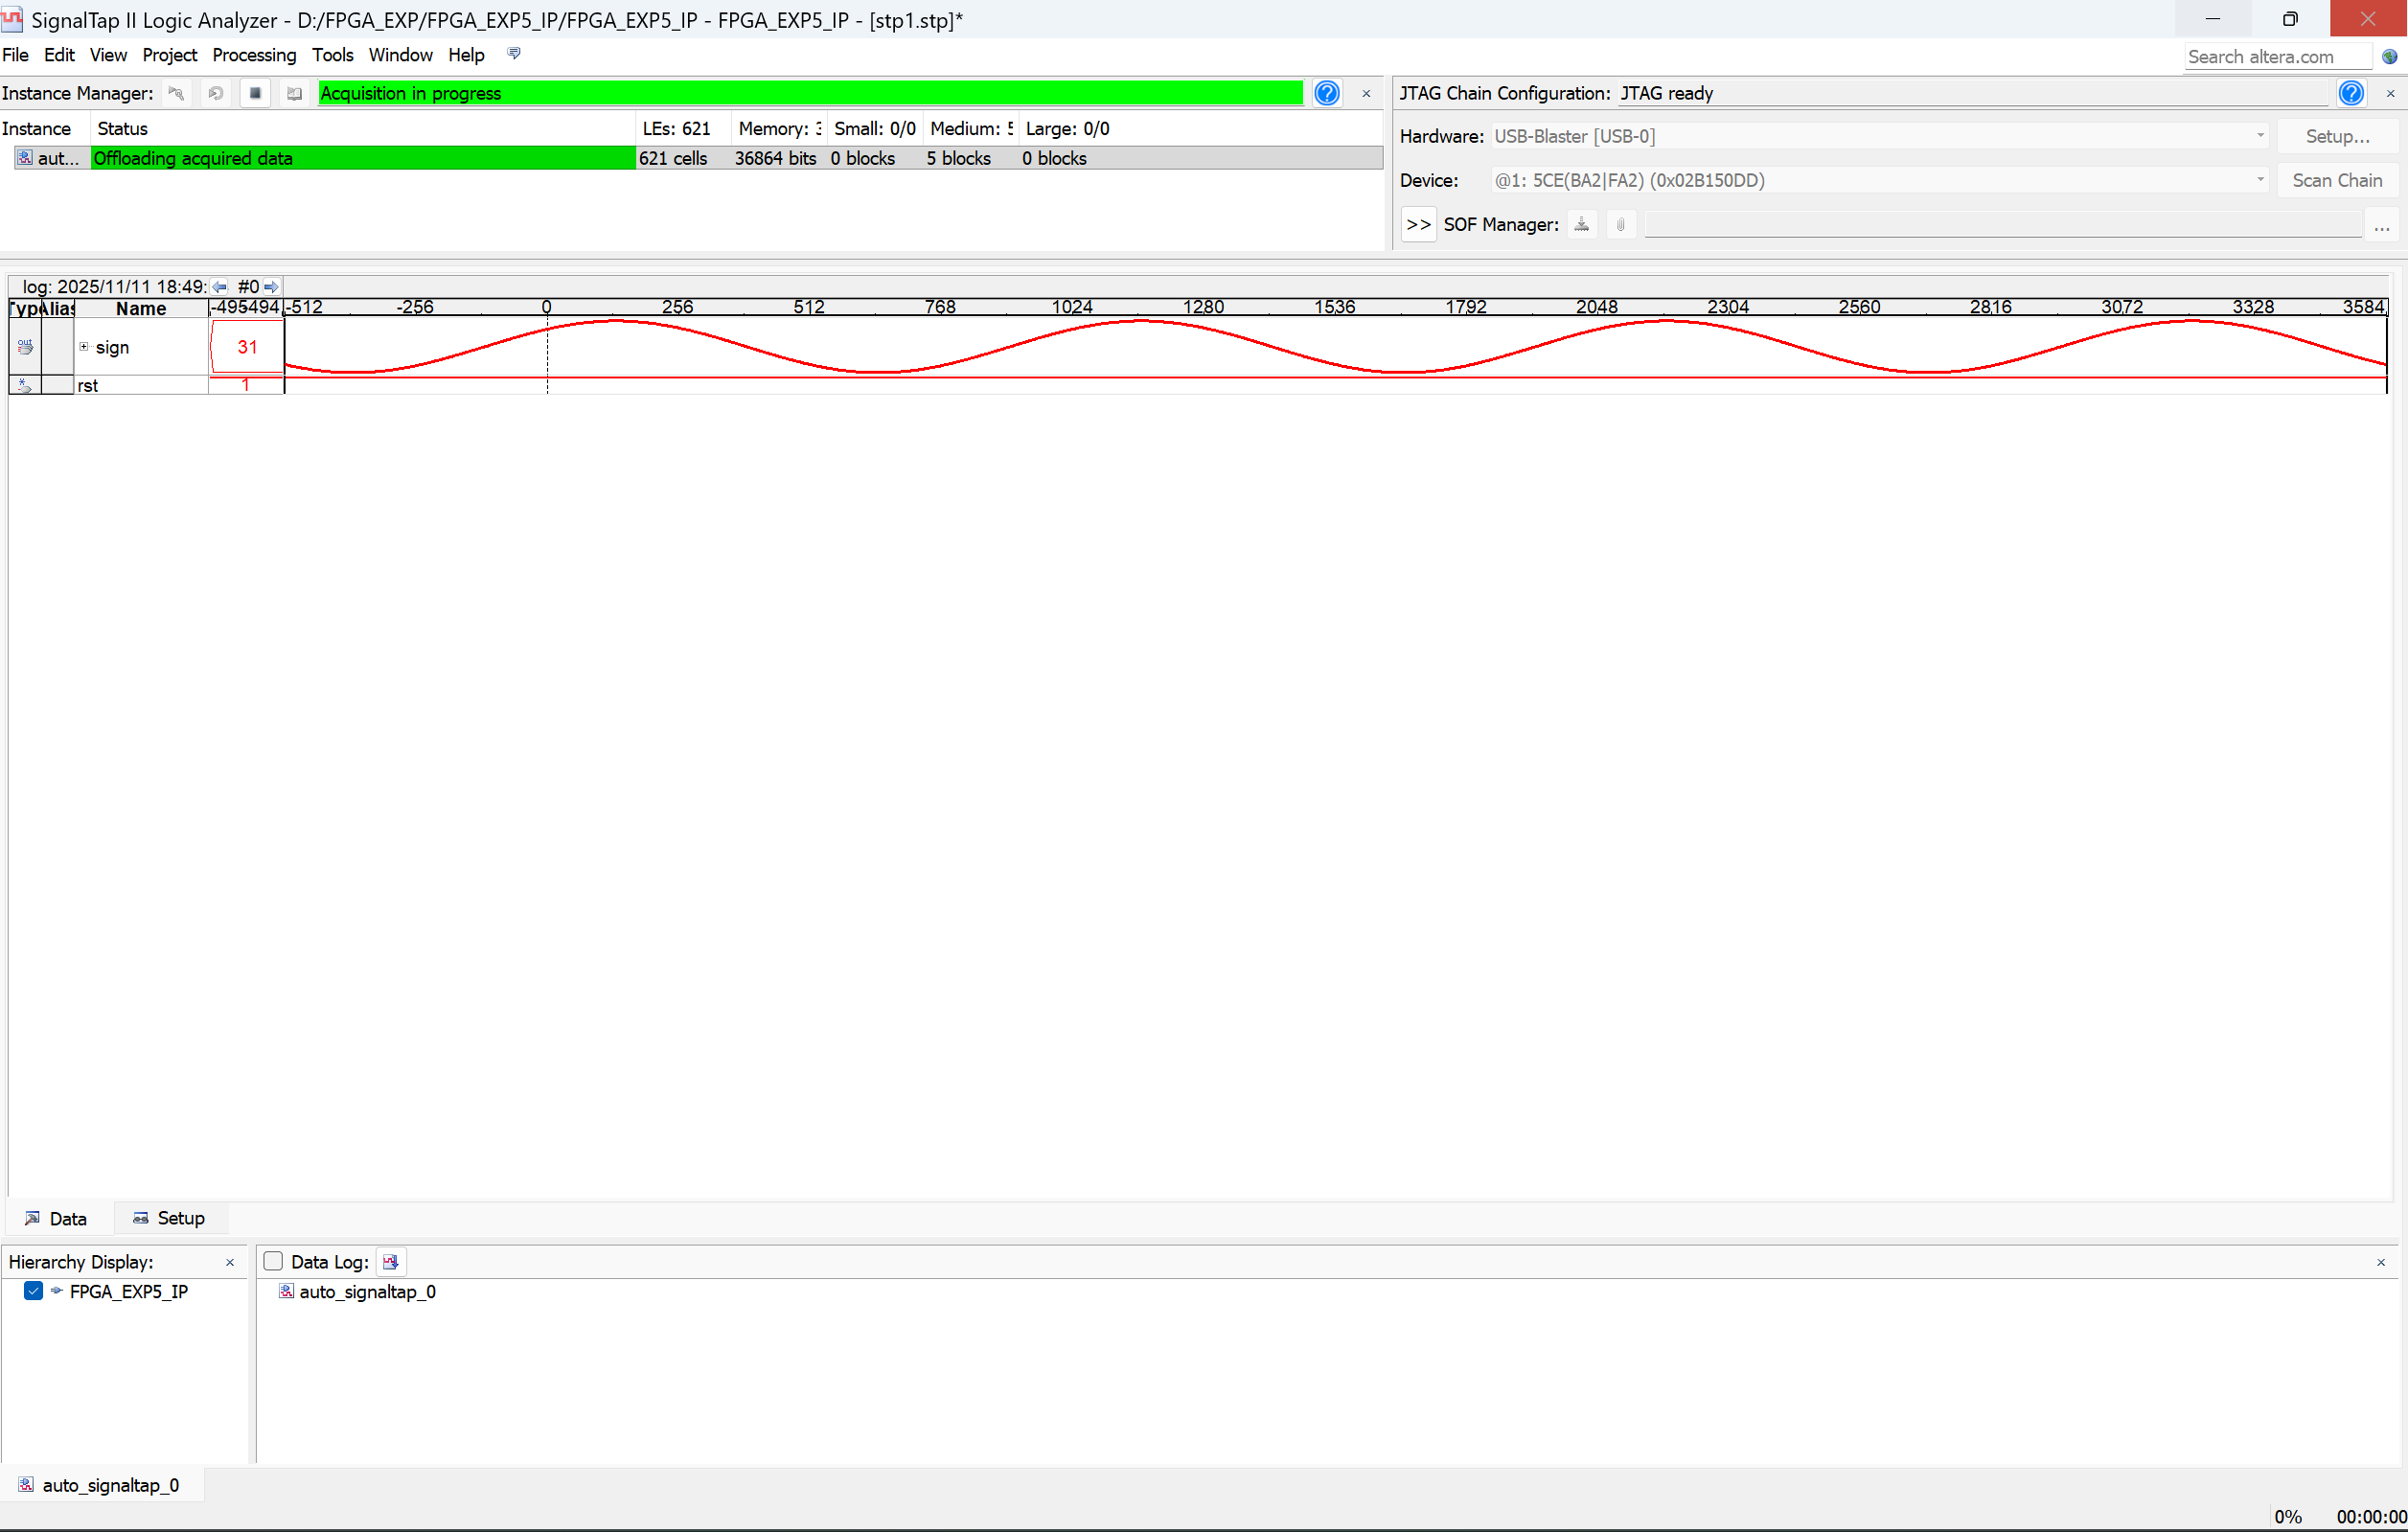
\includegraphics[width=\textwidth]{正弦.png}  % 图片的最大宽度为文本宽度
\end{figure}
\section*{2.蓝牙透传实验}
本实验是一个验证性实验，我们只需要跟着实验文档的步骤进行连接和配置即可实现两个PC端之间的通信。

在本次实验中，我的PC机作为从机与邻桌同学的PC机进行通信。经过配置后，成功实现了两个PC端之间的通信。

\begin{highlightedsection}{}
    六、实验总结
\end{highlightedsection}
本次实验较为简单，主要是验证性实验。通过本次实验，我了解了IP调用的基本方法，并且体验了蓝牙透传模块的使用方法。

本学期实验也就此结束，通过这几次实验，我对FPGA的设计流程有了更深入的了解，并且掌握了一些常用的模块设计方法。这些经验对我有很大的帮助和启发。

\end{document}